\documentclass[a4paper]{esannV2}
\usepackage{graphicx}
\usepackage{amssymb,amsmath,array,booktabs}
% Generated by experiments/make_numbers.py from results/summary.json. Do not edit.
\newcommand{\DSshortN}{1,417}
\newcommand{\DSshortSucc}{98.5}
\newcommand{\DSshortSNR}{115}
\newcommand{\DSshortMAE}{1.4\times 10^{-5}}
\newcommand{\DSshortSec}{2.5}
\newcommand{\DSshortFail}{21}
\newcommand{\DSshortFailAmb}{21}
\newcommand{\DSlongN}{191}
\newcommand{\DSlongSucc}{96.9}
\newcommand{\DSlongMAE}{4.0\times 10^{-6}}
\newcommand{\DSlongSNR}{127}
\newcommand{\DSlongSec}{37}
\newcommand{\DSlongMaxAudio}{35.0}
\newcommand{\DSlongestMAE}{1.3\times 10^{-4}}
\newcommand{\DSlongestFrames}{1,748}
\newcommand{\TFN}{600}
\newcommand{\TFSucc}{94.8}
\newcommand{\TFSNR}{63}
\newcommand{\TFSec}{8.5}
\newcommand{\TFMaxAudio}{9.6}
\newcommand{\GMmaeLo}{5.9}
\newcommand{\GMmaeHi}{8.0}
\newcommand{\GMsec}{2,973}
\newcommand{\GMn}{4}
\newcommand{\GMaudio}{2.3}
\newcommand{\AudMfccPrelimN}{39}
\newcommand{\AudMfccPrelimWEROrig}{2.2}
\newcommand{\AudMfccPrelimWERTrue}{4.0}
\newcommand{\AudMfccPrelimWERRec}{4.0}
\newcommand{\AudMfccPrelimWERGL}{6.5}
\newcommand{\AudMfccPrelimSpk}{90}
\newcommand{\AudMfccPrelimSim}{0.76}
\newcommand{\AudMfccPrelimSpeakers}{22}
\newcommand{\CkDsbegaEpbSeqSucc}{100}
\newcommand{\CkDsbegaEpbSeqSNR}{95}
\newcommand{\CkDsbegaEpbSeqN}{8}
\newcommand{\CkDsbegaLastLinearSucc}{98}
\newcommand{\CkDsbegaLastLinearSNR}{106}
\newcommand{\CkDsbegaLastLinearN}{60}
\newcommand{\CkDsbEpbaFinalbaaHLinearSucc}{98}
\newcommand{\CkDsbEpbaFinalbaaHLinearSNR}{105}
\newcommand{\CkDsbEpbaFinalbaaHLinearN}{60}
\newcommand{\CkDsbEpbaFinalbaaHSeqSucc}{100}
\newcommand{\CkDsbEpbaFinalbaaHSeqSNR}{102}
\newcommand{\CkDsbEpbaFinalbaaHSeqN}{12}
\newcommand{\CkDsbEpbLinearSucc}{98}
\newcommand{\CkDsbEpbLinearSNR}{100}
\newcommand{\CkDsbEpbLinearN}{60}
\newcommand{\CkDsbEpbSeqSucc}{100}
\newcommand{\CkDsbEpbSeqSNR}{106}
\newcommand{\CkDsbEpbSeqN}{12}
\newcommand{\CkDsbEpcLinearSucc}{98}
\newcommand{\CkDsbEpcLinearSNR}{103}
\newcommand{\CkDsbEpcLinearN}{60}
\newcommand{\CkDsbEpdLinearSucc}{98}
\newcommand{\CkDsbEpdLinearSNR}{104}
\newcommand{\CkDsbEpdLinearN}{60}
\newcommand{\CkDsbEpfLinearSucc}{98}
\newcommand{\CkDsbEpfLinearSNR}{107}
\newcommand{\CkDsbEpfLinearN}{60}
\newcommand{\CkDsbEpiLinearSucc}{98}
\newcommand{\CkDsbEpiLinearSNR}{107}
\newcommand{\CkDsbEpiLinearN}{60}
\newcommand{\CkDsbStepaLinearSucc}{98}
\newcommand{\CkDsbStepaLinearSNR}{117}
\newcommand{\CkDsbStepaLinearN}{60}
\newcommand{\CkDsbStepbaaaLinearSucc}{98}
\newcommand{\CkDsbStepbaaaLinearSNR}{102}
\newcommand{\CkDsbStepbaaaLinearN}{60}
\newcommand{\CkDsbStepbaaLinearSucc}{98}
\newcommand{\CkDsbStepbaaLinearSNR}{115}
\newcommand{\CkDsbStepbaaLinearN}{60}
\newcommand{\CkDsbStepdaaaLinearSucc}{98}
\newcommand{\CkDsbStepdaaaLinearSNR}{104}
\newcommand{\CkDsbStepdaaaLinearN}{60}
\newcommand{\CkDsbStepdaaLinearSucc}{98}
\newcommand{\CkDsbStepdaaLinearSNR}{104}
\newcommand{\CkDsbStepdaaLinearN}{60}
\newcommand{\CkTfegaLastSucc}{88}
\newcommand{\CkTfegaLastSNR}{54}
\newcommand{\CkTfegaLastN}{60}
\newcommand{\CkTfEpbSucc}{93}
\newcommand{\CkTfEpbSNR}{63}
\newcommand{\CkTfEpbN}{60}
\newcommand{\CkTfEpcgFinalbaaHSucc}{83}
\newcommand{\CkTfEpcgFinalbaaHSNR}{55}
\newcommand{\CkTfEpcgFinalbaaHN}{60}
\newcommand{\CkTfEpcgReconSucc}{91}
\newcommand{\CkTfEpcgReconSNR}{56}
\newcommand{\CkTfEpcgReconN}{80}
\newcommand{\CkTfEpfSucc}{67}
\newcommand{\CkTfEpfSNR}{52}
\newcommand{\CkTfEpfN}{27}
\newcommand{\CkTfStepaSucc}{93}
\newcommand{\CkTfStepaSNR}{64}
\newcommand{\CkTfStepaN}{60}
\newcommand{\CkTfStepdaaSucc}{90}
\newcommand{\CkTfStepdaaSNR}{63}
\newcommand{\CkTfStepdaaN}{60}
\newcommand{\CkTfStepdaaaSucc}{73}
\newcommand{\CkTfStepdaaaSNR}{48}
\newcommand{\CkTfStepdaaaN}{60}
\newcommand{\CkTfknownegaLastSucc}{93}
\newcommand{\CkTfknownegaLastSNR}{54}
\newcommand{\CkTfknownegaLastN}{60}
\newcommand{\CkTfknownEpcgFinalbaaHSucc}{90}
\newcommand{\CkTfknownEpcgFinalbaaHSNR}{55}
\newcommand{\CkTfknownEpcgFinalbaaHN}{60}
\newcommand{\CkTfknownEpfSucc}{77}
\newcommand{\CkTfknownEpfSNR}{49}
\newcommand{\CkTfknownEpfN}{60}
\newcommand{\CkTfknownStepdaaaSucc}{82}
\newcommand{\CkTfknownStepdaaaSNR}{48}
\newcommand{\CkTfknownStepdaaaN}{60}
\newcommand{\DfDsbClipaPabBlindSucc}{100}
\newcommand{\DfDsbClipaPabBlindMAE}{1.2\times 10^{-5}}
\newcommand{\DfDsbDropoutaPbLinearSucc}{98}
\newcommand{\DfDsbDropoutaPbLinearMAE}{7.5\times 10^{-6}}
\newcommand{\DfDsbDropoutaPcLinearSucc}{98}
\newcommand{\DfDsbDropoutaPcLinearMAE}{5.5\times 10^{-6}}
\newcommand{\DfDsbDropoutaPcSeqSucc}{0}
\newcommand{\DfDsbDropoutaPcSeqMAE}{7.5\times 10^{0}}
\newcommand{\DfDsbDropoutaPdLinearSucc}{98}
\newcommand{\DfDsbDropoutaPdLinearMAE}{4.0\times 10^{-6}}
\newcommand{\DfDsbDropoutaPfLinearSucc}{98}
\newcommand{\DfDsbDropoutaPfLinearMAE}{2.3\times 10^{-6}}
\newcommand{\DfDsbFbgKnownSucc}{10}
\newcommand{\DfDsbFbgKnownMAE}{2.9\times 10^{-2}}
\newcommand{\DfDsbNoisebEmbBlindSucc}{0}
\newcommand{\DfDsbNoisebEmbBlindMAE}{7.8\times 10^{0}}
\newcommand{\DfDsbNoisebEmbKnownSucc}{0}
\newcommand{\DfDsbNoisebEmbKnownMAE}{6.7\times 10^{0}}
\newcommand{\DfDsbNoisebEmcBlindSucc}{0}
\newcommand{\DfDsbNoisebEmcBlindMAE}{7.8\times 10^{0}}
\newcommand{\DfDsbNoisebEmcKnownSucc}{0}
\newcommand{\DfDsbNoisebEmcKnownMAE}{5.3\times 10^{0}}
\newcommand{\DfDsbNoisebEmdBlindSucc}{0}
\newcommand{\DfDsbNoisebEmdBlindMAE}{6.6\times 10^{-1}}
\newcommand{\DfDsbNoisebEmdKnownSucc}{0}
\newcommand{\DfDsbNoisebEmdKnownMAE}{6.6\times 10^{-1}}
\newcommand{\DfDsbNoisebEmeBlindSucc}{52}
\newcommand{\DfDsbNoisebEmeBlindMAE}{9.4\times 10^{-3}}
\newcommand{\DfDsbNoisebEmeKnownSucc}{52}
\newcommand{\DfDsbNoisebEmeKnownMAE}{9.4\times 10^{-3}}
\newcommand{\DfDsbNoisebEmfBlindSucc}{82}
\newcommand{\DfDsbNoisebEmfBlindMAE}{7.1\times 10^{-4}}
\newcommand{\DfDsbNoisebEmfKnownSucc}{82}
\newcommand{\DfDsbNoisebEmfKnownMAE}{7.1\times 10^{-4}}
\newcommand{\DfDsbNoisebEmgBlindSucc}{98}
\newcommand{\DfDsbNoisebEmgBlindMAE}{7.2\times 10^{-5}}
\newcommand{\DfDsbNoisebEmgKnownSucc}{98}
\newcommand{\DfDsbNoisebEmgKnownMAE}{7.2\times 10^{-5}}
\newcommand{\DfDsbNoisebEmhBlindSucc}{100}
\newcommand{\DfDsbNoisebEmhBlindMAE}{1.4\times 10^{-5}}
\newcommand{\DfDsbNoisebEmhKnownSucc}{100}
\newcommand{\DfDsbNoisebEmhKnownMAE}{1.4\times 10^{-5}}
\newcommand{\DfDsbPruneaPfBlindSucc}{0}
\newcommand{\DfDsbPruneaPfBlindMAE}{7.8\times 10^{0}}
\newcommand{\DfDsbPruneaPfKnownSucc}{0}
\newcommand{\DfDsbPruneaPfKnownMAE}{6.8\times 10^{0}}
\newcommand{\DfDsbPruneaPjjBlindSucc}{0}
\newcommand{\DfDsbPruneaPjjBlindMAE}{7.6\times 10^{0}}
\newcommand{\DfDsbPruneaPjjKnownSucc}{0}
\newcommand{\DfDsbPruneaPjjKnownMAE}{7.8\times 10^{0}}
\newcommand{\DfDsbPruneaPjBlindSucc}{0}
\newcommand{\DfDsbPruneaPjBlindMAE}{7.8\times 10^{0}}
\newcommand{\DfDsbPruneaPjKnownSucc}{0}
\newcommand{\DfDsbPruneaPjKnownMAE}{7.5\times 10^{0}}
\newcommand{\DfDsbQuantbgKnownSucc}{40}
\newcommand{\DfDsbQuantbgKnownMAE}{1.3\times 10^{-2}}
\newcommand{\DfDsbQuantiKnownSucc}{0}
\newcommand{\DfDsbQuantiKnownMAE}{6.1\times 10^{0}}
\newcommand{\DfDsbSignKnownSucc}{0}
\newcommand{\DfDsbSignKnownMAE}{7.6\times 10^{0}}
\newcommand{\DfDsbTrainedDropoutaPcLinearSucc}{98}
\newcommand{\DfDsbTrainedDropoutaPcLinearMAE}{2.2\times 10^{-5}}
\newcommand{\DfTfNoisebEmdKnownSucc}{0}
\newcommand{\DfTfNoisebEmdKnownMAE}{4.8\times 10^{-1}}
\newcommand{\DfTfPruneaPjKnownSucc}{0}
\newcommand{\DfTfPruneaPjKnownMAE}{8.0\times 10^{-1}}
\newcommand{\DfTfTrainmodeSucc}{95}
\newcommand{\DfTfTrainmodeMAE}{2.9\times 10^{-4}}
\newcommand{\FlLocalSgdUttsbStepsbLraPabMAE}{4.5\times 10^{-3}}
\newcommand{\FlLocalSgdUttsbStepsbLraPabSucc}{85}
\newcommand{\FlLocalSgdUttsbStepscLraPabMAE}{2.5\times 10^{-3}}
\newcommand{\FlLocalSgdUttsbStepscLraPabSucc}{90}
\newcommand{\FlLocalSgdUttsbStepsfLraPabMAE}{2.2\times 10^{-3}}
\newcommand{\FlLocalSgdUttsbStepsfLraPabSucc}{85}
\newcommand{\FlLocalSgdUttsbStepsbaLraPabMAE}{4.4\times 10^{-3}}
\newcommand{\FlLocalSgdUttsbStepsbaLraPabSucc}{100}
\newcommand{\FlLocalSgdUttsbStepsbaLraPbMAE}{2.6\times 10^{-4}}
\newcommand{\FlLocalSgdUttsbStepsbaLraPbSucc}{100}
\newcommand{\FlLocalSgdUttsbStepsfaLraPabMAE}{5.4\times 10^{-3}}
\newcommand{\FlLocalSgdUttsbStepsfaLraPabSucc}{90}
\newcommand{\FlBatchUttscStepsbLraPbMAE}{1.6\times 10^{-3}}
\newcommand{\FlBatchUttscStepsbLraPbSucc}{100}
\newcommand{\FlSgdMomentumUttsbStepsbaLraPbMAE}{1.0\times 10^{-4}}
\newcommand{\FlSgdMomentumUttsbStepsbaLraPbSucc}{95}
\newcommand{\FlSgdWeightDecayUttsbStepsbaLraPbMAE}{5.2\times 10^{-4}}
\newcommand{\FlSgdWeightDecayUttsbStepsbaLraPbSucc}{100}
\newcommand{\FlAdamUttsbStepsbLraPaabMAE}{7.4\times 10^{0}}
\newcommand{\FlAdamUttsbStepsbLraPaabSucc}{0}
\newcommand{\FlAdamUttsbStepsbaLraPaabMAE}{7.4\times 10^{0}}
\newcommand{\FlAdamUttsbStepsbaLraPaabSucc}{0}
\newcommand{\FlBatchShortUttseStepsbLraPbMAE}{5.9\times 10^{-4}}
\newcommand{\FlBatchShortUttseStepsbLraPbSucc}{90}
\newcommand{\FlBatchShortUttsiStepsbLraPbMAE}{1.3\times 10^{-3}}
\newcommand{\FlBatchShortUttsiStepsbLraPbSucc}{80}
\newcommand{\FlBatchShortUttsbgStepsbLraPbMAE}{1.1\times 10^{-3}}
\newcommand{\FlBatchShortUttsbgStepsbLraPbSucc}{85}
\newcommand{\FlLocalEpochsBatchbUttseStepsiLraPbMAE}{5.5\times 10^{-4}}
\newcommand{\FlLocalEpochsBatchbUttseStepsiLraPbSucc}{90}
\newcommand{\FlLocalEpochsBatchbUttsiStepsbgLraPbMAE}{1.1\times 10^{-3}}
\newcommand{\FlLocalEpochsBatchbUttsiStepsbgLraPbSucc}{90}
\newcommand{\CfdfbcCov}{92}
\newcommand{\CfdfbcSNR}{14}
\newcommand{\CfdfbcN}{1}
\newcommand{\CfdfbcsingleCov}{9}
\newcommand{\CfdfbcsingleSNR}{16}
\newcommand{\CfdfbcsingleN}{10}
\newcommand{\TrdsbWER}{40.7}
\newcommand{\TrdsbegaWER}{25.5}
\newcommand{\TrtfWER}{24.0}
\newcommand{\TrtfegaWER}{13.3}
\newcommand{\TrDSsucc}{98.3}
\newcommand{\TrDSwer}{41}
\newcommand{\DropSucc}{98.3}
\newcommand{\TrTFsucc}{83}
\newcommand{\TrTFknownSucc}{90}
\newcommand{\TrTFwer}{24}
\newcommand{\WERrec}{3.8}
\newcommand{\WERorig}{3.0}
\newcommand{\SpkRec}{98}
\newcommand{\Speakers}{40}
\newcommand{\PruneSucc}{0}
\newcommand{\SignSucc}{0}
\newcommand{\ConfCov}{9}
\newcommand{\ConfSNR}{16}
\newcommand{\ConfN}{10}
\newcommand{\GMmae}{5.9 to 8.0}
\newcommand{\SilencePct}{1.5}
\newcommand{\DropAllSucc}{98}
\newcommand{\WerShort}{3.8}
\newcommand{\WerOrigShort}{3.0}
\newcommand{\SpkShort}{98}
\newcommand{\SpkOrigShort}{99}
\newcommand{\AudNShort}{197}
\newcommand{\WerGLShort}{5.1}
\newcommand{\WerLong}{4.2}
\newcommand{\WerOrigLong}{3.4}
\newcommand{\SpkLong}{100}
\newcommand{\SpkOrigLong}{100}
\newcommand{\AudNLong}{57}
\newcommand{\WerTf}{4.2}
\newcommand{\WerOrigTf}{3.8}
\newcommand{\SpkTf}{99}
\newcommand{\SpkOrigTf}{99}
\newcommand{\AudNTf}{186}
\newcommand{\WerDrop}{4.7}
\newcommand{\WerOrigDrop}{2.4}
\newcommand{\SpkDrop}{98}
\newcommand{\SpkOrigDrop}{100}
\newcommand{\AudNDrop}{58}
\newcommand{\WerTfTr}{3.7}
\newcommand{\WerOrigTfTr}{2.3}
\newcommand{\SpkTfTr}{99}
\newcommand{\SpkOrigTfTr}{100}
\newcommand{\AudNTfTr}{80}


\voffset 0 cm \hoffset -0.14 cm \addtolength{\textwidth}{0cm}
\addtolength{\textheight}{0cm}\addtolength{\leftmargin}{0cm}

\begin{document}
% TODO(Taka): confirm the author list before submission.
\title{Frames in the span: exact recovery of long-form speech from federated ASR updates}

\author{Taka Khoo
\vspace{.3cm}\\
Dartmouth College - Thayer School of Engineering \\
Hanover, NH - USA
}

\maketitle

\begin{abstract}
Federated speech recognition shares model updates in place of audio. We show that for models
whose first layer applies one linear map to overlapping windows of feature frames, a single
update contains the features. The rows of the first-layer gradient span the windows, the
overlap makes membership in that span a linear system, and a banded solve returns the
utterance: \DSshortSucc\% of \DSshortN{} LibriSpeech utterances up to 6.2\,s at
\DSshortSNR\,dB SNR, without transcript, length, loss or optimisation. The system is
solvable up to $(k-s)F$ windows. Deeper layers extend the attack to 35\,s. It survives
local SGD, batching, dropout and training.
\end{abstract}

\section{Introduction}

Federated learning (FL) trains a model on client devices and returns updates to a server
\cite{mcmahan2017communication}. For automatic speech recognition (ASR) the appeal is plain: the audio
never leaves the device \cite{guliani2021training,pelikan2025enabling}. Gradient inversion
\cite{zhu2019dlg,geiping2020inverting} asks how much of the input the update still reveals.

For speech the answers so far come from optimisation. Dang et al.\ \cite{dang2022speaker} reconstruct
DeepSpeech \cite{hannun2014deep} features with a zeroth-order search, given the transcript and length of
short utterances, and identify the speaker in 34\% of cases; dropout brings this to 0\%. Later work
matches gradients of small classifiers \cite{li2023speech,ovi2024gradient}, reaching long audio by
segmenting it \cite{zeng2025recover}, or matches DeepSpeech gradients through the CTC loss
\cite{graves2006connectionist,bui2025reconstructing}. These attacks are slow, need side information, and
their failures under dropout, local training or long inputs are read as evidence that realistic FL is
hard to invert \cite{du2025sok}.

We take the algebraic route opened for text and images by DAGER \cite{petrov2024dager}, SPEAR
\cite{dimitrov2024spear} and TIGER \cite{kalikman2026tiger}: the gradient of a linear layer is low rank
and its row space is the span of the layer's inputs. Our observation is that speech front ends make this
span unusually easy to read. Frames of one utterance act as a batch, and each frame is seen through a
\emph{window} that overlaps its neighbours. The overlap is what turns span membership into a linear
system. Contributions:
\begin{itemize}
\item a closed-form attack on the first layer with a capacity law, $(k-s)F$ windows for kernel $k$,
stride $s$ and $F$ features, verified on four front ends;
\item a sequential decoder that uses the spans leaked by deeper layers and recovers every test
utterance length we tried, up to \DSlongMaxAudio\,s;
\item evidence that the leak survives what FL adds (local SGD, momentum, weight decay, batches,
clipping, dropout) and training, with a noise threshold predicted by a singular value;
\item an account of what does stop it: local Adam, pruning, noise, narrow or non-overlapping first layers.
\end{itemize}

\section{The span leak}

\textbf{Setting.} A client holds features $X=(x_1,\dots,x_T)$, $x_t\in\mathbb{R}^F$. The first layer
reads windows $c_p(X)=[x_{ps-a},\dots,x_{ps-a+k-1}]\in\mathbb{R}^{kF}$, $p=1..P$, with zeros outside
$1..T$, and outputs $Wc_p+b$, $W\in\mathbb{R}^{H\times kF}$. DeepSpeech-1 splices $c$ context frames on
each side ($k=2c+1$, $s=1$); the Transformer encoder of \cite{pelikan2025enabling} uses a convolution
with $k=7$, $s=3$ on $F=80$ log-mel bins. The server knows the model and receives the update.

\textbf{Span.} For any loss $L$ and any later layers, with $g_p=\partial L/\partial(Wc_p+b)$,
\[
\nabla_W L=\sum_{p=1}^{P} g_p\,c_p^{\top},\qquad \nabla_b L=\sum_{p=1}^{P} g_p .
\]
The row space of $M=[\nabla_W L\mid\nabla_b L]$ lies in $\mathcal{S}=\mathrm{span}\{[c_p,1]\}$ and
equals it when the $g_p$ are linearly independent, which needs $H\ge P$ and holds generically after a
nonlinearity. Then $\mathrm{rank}\,M$ is the number of independent windows: \emph{the update reveals the
length of the utterance}.

\textbf{Linear system.} Let $\Pi^{\perp}$ project onto $\mathcal{S}^{\perp}$, obtained from the SVD of
$M$. The true features satisfy $\Pi^{\perp}[c_p(X),1]=0$ for all $p$. Since $c_p$ is linear in $X$, this
is a linear system; its normal matrix is block-banded with bandwidth $kF$, and we solve it by banded
Cholesky. Counting gives a necessary condition for uniqueness: $P(kF+1-P)$ equations for about $sPF$
unknowns, hence
\[
P\;\le\;(k-s)F+1 .
\]
Without overlap ($k=s$) every window may be any vector of $\mathcal{S}$ and nothing is identified.

\textbf{Local training.} After $K$ local SGD steps the server computes
$(W_0-W_K)/\eta=\sum_{j}\sum_p g_p^{(j)}c_p^{\top}$. The windows do not depend on the weights, so the row
space is the same $\mathcal{S}$. Momentum reweights the terms; weight decay adds a known multiple of
$W_0$ that the server removes. A batch adds the windows of all its utterances to one span. Clipping
rescales $M$. Dropout placed after the first layer changes $g_p$ only.

\textbf{Noise.} If the update is $M+E$ with i.i.d.\ Gaussian $E$ of standard deviation $\sigma$,
$\|E\|_2\approx\sigma(\sqrt{H}+\sqrt{kF+1})$, and by Wedin's theorem the span is perturbed by an angle
of order $\rho=\|E\|_2/s_P(M)$, with $s_P$ the weakest signal singular value. The attack should degrade
linearly in $\rho$ and fail near $\rho=1$.

\section{Beyond the first layer}

Past the capacity the first-layer span fills its space. The next layers still leak. In DeepSpeech-1
the second and third layers and the LSTM input are linear maps of $h_1(c_t)$, $h_2(c_t)$, $h_3(c_t)$,
clipped-ReLU functions of one window with 2{,}048 to 4{,}096 units, and their gradients have row space
$\mathrm{span}\{[h_\ell(c_t),1]\}$ of dimension $T$ for $T$ up to the layer width. The nonlinearity is
what raises the capacity: a linear network would leak the same 339-dimensional span at every layer.

A candidate window $c$ can be tested: the residual $r(c)=\Pi_\ell^{\perp}[h_\ell(c),1]$ vanishes on true
windows, and generically only there, since a $kF$-dimensional manifold meets a $T$-dimensional subspace
of a much larger space in isolated points. The test does not say \emph{which} frame a window is, so
descending on all frames jointly stalls. The padding breaks the symmetry. The first window holds $c$ zero
frames followed by $x_1,\dots,x_{c+1}$: we solve for it by Levenberg--Marquardt, starting from the opening
frames of public utterances. Every later window shares all but one frame with its predecessor, so each
step has only $F$ unknowns. We use the spans of the second and third layers (the LSTM-input span is noisier and is needed only beyond 37\,s), re-fit the last 26 frames jointly every 8 steps to stop drift, and stop
when six consecutive decoded frames are zero, which is the padding at the far end. The length is
therefore an output of the attack. A final joint refinement polishes all frames.

\section{Experiments}

\textbf{Setup.} LibriSpeech \cite{panayotov2015librispeech} test-clean, one float32 gradient of the CTC
loss per utterance. DeepSpeech-1: 26 MFCCs at 50\,Hz, $c=6$, 2{,}048 units, clipped ReLU. Transformer-CTC:
80 log-mel bins at 100\,Hz, per-utterance normalisation, a 1-D convolution from 80 to 1{,}536 channels ($k=7$, $s=3$) with a gated
linear unit, 12 blocks. Both are attacked at random initialisation and at checkpoints of training on 100\,h.
The attacker receives the update and the model only. An utterance counts as recovered if the mean
absolute error (MAE) is below $10^{-2}$ (MFCCs have mean magnitude 8) or the SNR exceeds 30\,dB (log-mel).

\begin{table}[t]
\centering\footnotesize
\begin{tabular}{@{}llrrrr@{}}
\toprule
Target & Attack & $n$ & Length (s) & Recovered & SNR (dB)\\
\midrule
DeepSpeech-1 & closed form & \DSshortN & 1.3--6.2 & \DSshortSucc\% & \DSshortSNR\\
DeepSpeech-1 & sequential & \DSlongN & 6.3--\DSlongMaxAudio & \DSlongSucc\% & \DSlongSNR\\
DeepSpeech-1, trained & closed form & 60 & $\le$6.2 & \TrDSsucc\% & \\
\quad + dropout 0.2 & closed form & 60 & $\le$6.2 & \DropSucc\% & \\
Transformer-CTC & closed form & \TFN & $\le$9.6 & \TFSucc\% & \TFSNR\\
Transformer-CTC, trained & closed form$^\dagger$ & 60 & $\le$9.6 & \TrTFknownSucc\% & \\
Gradient matching \cite{bui2025reconstructing} & 2{,}000 steps$^\ddagger$ & \GMn & \GMaudio & 0\% & $<$3\\
\bottomrule
\end{tabular}
\caption{One update per utterance. Median SNR of the recovered features. $^\dagger$length given
(\TrTFsucc\% without). $^\ddagger$transcript and length given; \GMsec\,s per utterance against
\DSshortSec\,s for the closed form.}\label{tab:main}
\end{table}

\begin{figure}[t]
\centering
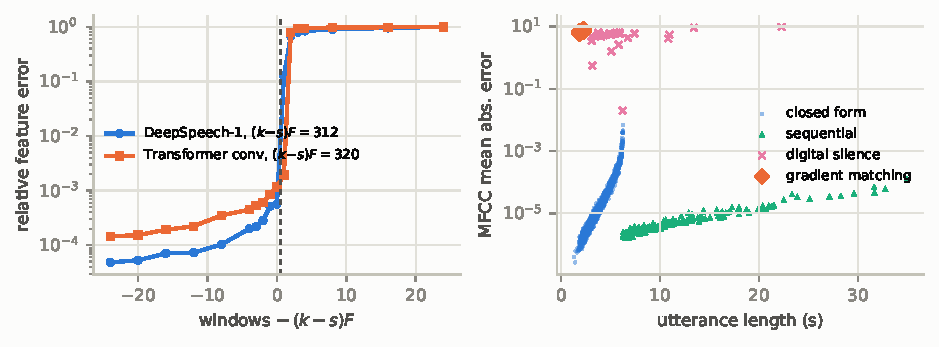
\includegraphics[width=\textwidth]{../../docs/figures/paper_main.pdf}
\caption{Left: error of the closed form around the predicted capacity (real features cropped to an
exact length). Right: error against utterance length for every attacked utterance.}\label{fig:main}
\end{figure}

\textbf{Closed form.} Table~\ref{tab:main} and Fig.~\ref{fig:main}. On DeepSpeech-1 the attack recovers
\DSshortSucc\% of the \DSshortN{} utterances that fit in the first layer, with median MAE
$\DSshortMAE$, and reads the length exactly from the rank. All \DSshortFail{} failures are flagged by a
uniqueness test in the solver: these recordings contain runs of bit-identical frames (digital silence),
which make windows identical and the solution non-unique. On the Transformer front end \TFSucc\% of
\TFN{} utterances up to 9.6\,s are recovered. The capacity is sharp: on four front ends the error stays
below $10^{-3}$ up to $(k-s)F$ windows (312, 468, 320, 240) and reaches order one within two windows.

\textbf{Long utterances.} The sequential decoder recovers \DSlongSucc\% of \DSlongN{} utterances
between 6.3 and \DSlongMaxAudio\,s (median MAE $\DSlongMAE$), including the longest utterance of the
set, \DSlongestFrames{} frames. The failures are again digital silence. Trained checkpoints decode equally well (12 of 12).

\textbf{Baseline.} Gradient matching on the output layer, through a CTC loss that can be differentiated
twice and with transcript and length given, ends at MAE \GMmae{} after \GMsec\,s on 2\,s utterances: the gradient is
matched (cosine distance below $10^{-2}$) and the features are not, as the output-layer gradient has
rank at most 29.

\textbf{What the server receives.} With the first-layer update computed from weight differences, the
closed form is unaffected by 1 to 50 local SGD steps, momentum and weight decay (median MAE between
$10^{-4}$ and $6\cdot10^{-3}$; the floor is float32 rounding in the subtraction and shrinks with larger
steps). Batches of 2 to 16 utterances within capacity are recovered when their lengths are given.
Dropout up to 0.5 on the client leaves \DropAllSucc\% recovered, which contradicts the protection
reported for optimisation attacks \cite{dang2022speaker}. Training does not help: DeepSpeech-1
checkpoints from step 0 to \TrDSwer\% word error rate are all recovered at \TrDSsucc\%.

\textbf{Audio.} A small network maps recovered features to the mel input of a public HiFi-GAN
\cite{kong2020hifigan}, trained on speakers disjoint from the test set. Whisper \cite{radford2023robust}
transcribes the result at \WerShort\% word error rate (original audio: \WerOrigShort\%), and ECAPA
embeddings \cite{desplanques2020ecapa} identify the speaker among \Speakers{} for \SpkShort\% of
reconstructions.

\textbf{What stops it.} Local Adam (per-coordinate rescaling), magnitude pruning of half the entries and
sign compression destroy the low-rank structure (0\% recovered). Gaussian noise behaves as predicted:
the error is proportional to $\rho$ and the attack fails near $\rho=1$, which for these utterances is a
noise level near $10^{-3}$ of the gradient RMS. First layers that are narrow or have no overlap do not
leak a usable span: we measured the gradient rank of the first layers of pretrained Whisper and wav2vec
2.0 \cite{baevski2020wav2vec}, DeepSpeech-2 \cite{amodei2015deep} and QuartzNet \cite{kriman2020quartznet};
all are saturated. Some leak one layer later (wav2vec 2.0 feature projection, the linear layer after
Conformer subsampling \cite{gulati2020conformer}), where a decoder analogous to ours finds true
windows but recovers only \ConfCov\% of the frames on average (\ConfSNR\,dB) before its chains stall; we
count that as a negative result for now. Dropout also stops the sequential decoder, since deeper layers
see the dropped activations.

\section{Conclusion}

A wide linear layer over overlapping feature windows makes one federated update equivalent to the
utterance, up to a capacity that we can write down. The defences that work are the ones that break the
low-rank structure or exceed the capacity; dropout, clipping, local SGD and training do neither. Central
differential privacy adds noise after aggregation and does not protect a client from the server itself.
Code, per-utterance results and audio: \texttt{github.com/takakhoo/unsplice}.

\begin{footnotesize}
\bibliographystyle{unsrt}
\bibliography{../refs}
\end{footnotesize}

\end{document}
